%
% General structure for the revdetua class:
%
\documentclass[portugues,final]{revdetua}
\usepackage[portuguese]{babel}
\usepackage{listingsutf8}
\usepackage[utf8]{inputenc}
\usepackage[T1]{fontenc}
\usepackage{graphicx}
\usepackage{hyperref}
\usepackage{wrapfig}
\usepackage{float}
\usepackage{natbib}
\usepackage{color}
\usepackage{eurosym}
%
% Valid options are:
%
%   longpaper --------- \part and \tableofcontents defined
%   shortpaper -------- \part and \tableofcontents not defined (default)
%
%   english ----------- main language is English (default)
%   portugues --------- main language is Portuguese
%
%   draft ------------- draft version
%   final ------------- final version (default)
%
%   times ------------- use times (postscript) fonts for text
%
%   mirror ------------ prints a mirror image of the paper (with dvips)
%
%   visiblelabels ----- \SL, \SN, \SP, \EL, \EN, etc. defined
%   invisiblelabels --- \SL, \SN, \SP, \EL, \EN, etc. not defined (default)
%
% Note: the final version should use the times fonts
% Note: the really final version should also use the mirror option
%

\begin{document}

% Note: the month must be in Portuguese

\title{\textbf{Jogo de Xadrez implementado em OpenGL} \\ Computação Visual\\Universidade de Aveiro}
\author{Diogo Silva 60337}
\maketitle

\begin{resumo} % Note: in Portuguese
  ...
\end{resumo}

\begin{palavraschave} % Note: in Portuguese (optional)
  ...
\end{palavraschave}

\section{Estrutura da Aplicação}

A aplicação do jogo inicialmente encontrava-se em C, tal como foi sugerido nas aulas, mas devido à necessidade de introduzir o conceito de herança nas peças de Xadrez, passou-se tudo para C++ e realizou-se o desenvolvimento a partir daí.\\

Para compilar o código existe um Makefile disponível no qual foi criado para Linux, apesar de o executável estar disponível de qualquer das formas.

FALTA FALAR DA COMPILAÇÃO MELHOR

\subsection{Engine do Jogo de Xadrez}

O motor do jogo tem as seguintes funcionalidades como:
\begin{enumerate}
\item{Obter lista das referências para cada peça}
\item{Verificar se o jogo já acabou e quem ganhou}
\item{Verificar de quem é a vez de jogar}
\item{Realizar um movimento}
\item{Mostrar movimentos possíveis de uma peça}
\end{enumerate}

Tal como mostra a figura seguinte, pode-se verificar que estas funcionalidades são acedidas facilmente através da classe Chess.

\begin{figure}[H]
\centerline{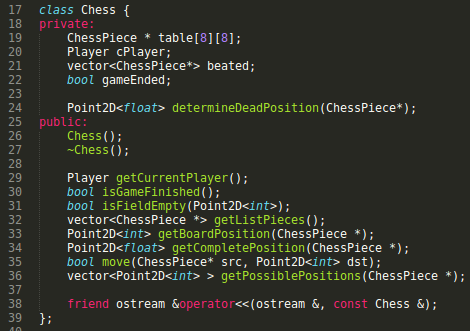
\includegraphics[width=230pt]{images/chess.png}}
\caption{Implementação do Chess}
\label{img:complete}
\end{figure}

Por sua vez, a classe Chess contém uma matrix de 8 por 8 (64 lugares) em que no ínicio, estão 32 ocupadas e as restantes apontar para NULL, esta matrix é uma matrix de referências de Peças de Xadrez, mais precisamento, objectos do tipo ChessPiece (descritos detalhadamente na secção seguinte).

\subsubsection{Peças do Xadrez}

As peças de Xadrez têm um módulo do qual permite destinguir a qual jogador pertence a peça, o tipo da peça (se é um Rei, um Cavalo, etc..). Consecutivamente, também é o que permite destinguir movimentos das peças.\\

Todas as peças herdam uma classe principal chamada ChessPiece, que contém as funcionalidades referidas anteriomente, tal como mostra a figura seguinte:

\begin{figure}[H]
\centerline{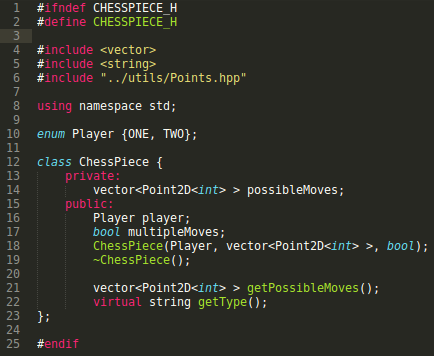
\includegraphics[width=230pt]{images/chesspiece.png}}
\caption{Implementação do ChessPiece}
\label{img:complete}
\end{figure}

Tal como foi referido, todas as peças têm de indicar na sua inicialização a lista de movimentos possíveis, se são movimentos multíplos ou não e o jogador a qual pertence, na figura seguinte pode-se ver o exemplo da implementação da Rainha, em que mostra que os movimentos possíveis são em todas as casas as sua volta e são movimentos multíplos.

\begin{figure}[H]
\centerline{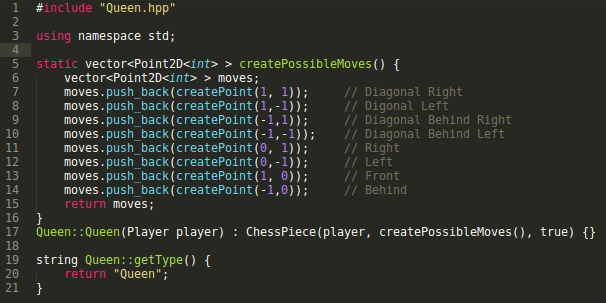
\includegraphics[width=230pt]{images/queen.png}}
\caption{Implementação da Peça Rainha}
\label{img:complete}
\end{figure}

\subsection{Desenvolvimento OpenGL}

Relativamente a implementação da parte gráfica da aplicação, decidiu-se dar continuação a estrutura já existentes das aulas, tendo os seguintes ficheiros:
\begin{enumerate}
\item{init.cpp, que inicia todos os modelos, fontes de luz, estruturas, janela e callbacks}
\item{models.cpp, que permite ler os ficheiros obj do formato oficial}
\item{globals.cpp, contém algumas variaveis globais para permitir fácil manipulação durante o uso de callbacks}
\item{callbacks.cpp, este ficheiro é o que trata de reescrever a imagem, trata também ainda dos movimentos do rato e cliques do teclado}
\item{shaders.cpp, este ficheiro é o que carrega o vertex e o fragment shader}
\end{enumerate}

Para além deste ainda foram criados dois ficheiros, um LightModel.cpp que contém apenas todas as caracteristicas necessárias para a representação de um foco de iluminação, tais como, posição do foco, intensidade do foco e intensidade da luz ambiente.
O outro ficheiro, é o ficheiro GraphicModelChess.cpp que contém as caracteristicas gráficas de cada modelo de Xadrez (este ficheiro é descrito detalhamente na secção seguinte).

\subsubsection{Modelos}

{\large Estrutura do GraphicModelChess}

A classe GraphicModelChess contém todas as caracteristicas gráficas de cada modelo:
\begin{enumerate}
\item{Número de vertíces}
\item{Lista de vertíces}
\item{Lista das normais}
\item{Valores de deslocamento, rotação e de redimensionamento}
\item{Coeficiente Ambiente, Difusão, Especular e Phong}
\end{enumerate}

Para além deste valores, ainda contém uma referência para o respectivo modelo de Xadrez, ou seja, objecto ChessPiece.

A figura seguinte mostra o cabeçalho deste ficheiro:

\begin{figure}[H]
\centerline{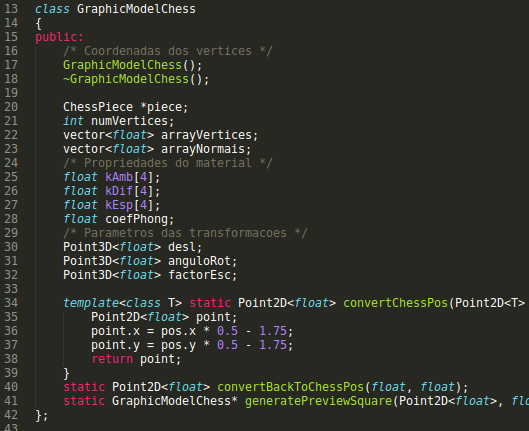
\includegraphics[width=230pt]{images/graphicmodelchess.png}}
\caption{Cabeçalho do GraphicModelChess}
\label{img:complete}
\end{figure}

Ainda se pode verificar a existência de 3 funções estáticas, duas das quais servem para converter coordenadas do tabuleiro de Xadrez para coordenadas do mundo 3D, e vice-versa. A outra função serve para gerar modelos quadrados que vão servir para representar todas as alternativas possíveis de cada movimento.

{\large Load de cada modelo de Xadrez}

As peças do Xadrez foram retiradas de modelos já existentes num projecto Open Source \url{https://code.google.com/p/pwag-chessboard/}, desse projecto foram retirados do directório /trunk/Chess/Chess/Models.\\

Sendo que esses modelos foram todos optimizados usando o programa Blender de maneira a ficarem da forma pretendida, tal como, colocar a base no plano xOy, ou seja, z = 0.

Após a recolocação dos modelos, foram todos exportados para ficheiros .obj no formato oficial.

Apesar de fazer a leitura do modelo oficial dos ficheiros obj, apenas são carregados os vertices, as normais e as faces, deixando de foram os vertices das texturas.

O load genérico dos ficheiros obj encontra-se em /src/models.cpp.

\subsubsection{Shaders}

Inicialmente os shaders apenas estavam a ser usados para a representação das cores, não fazendo qualquer procesamento na gráfica, mas houve a necessidade de implementar a iluminação nos shaders devido ao tentar fazer uma animação mais complexa e notar-se que a imagem não era completamente fluída porque o tempo que o CPU demorava a fazer os calculos das iluminações de cada vertice era superior ao tempo da rotação, verificando-se um delay no movimento.\\

Sendo assim, havia duas opções, tornar a animação mais rudimentar, ou passar a iluminação para os shaders (fazendo com que a gráfica processa-se a animação).

\begin{figure}[H]
\centerline{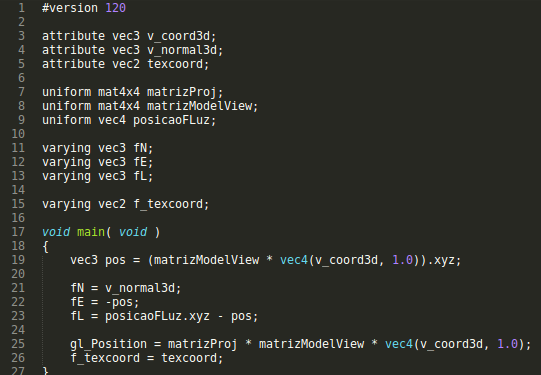
\includegraphics[width=230pt]{images/vertexshader.png}}
\caption{Vertex Shader}
\label{img:complete}
\end{figure}

Como se pode verificar no vertex shader é feito os calculos do ponto relativamente a um vertice, a sua posição, consoante a matrix projecção e o modelo, para além disso, ainda é calculado alguma fracções que vão ser usadas mais tarde pelo fragment shader, estas precisam de ser calculadas no vertex porque a iluminação depende da posição do vertice e do foco de iluminação.\\

Ainda se pode verificar que as coordenadas das texturas são passadas para o fragment shader.

\begin{figure}[H]
\centerline{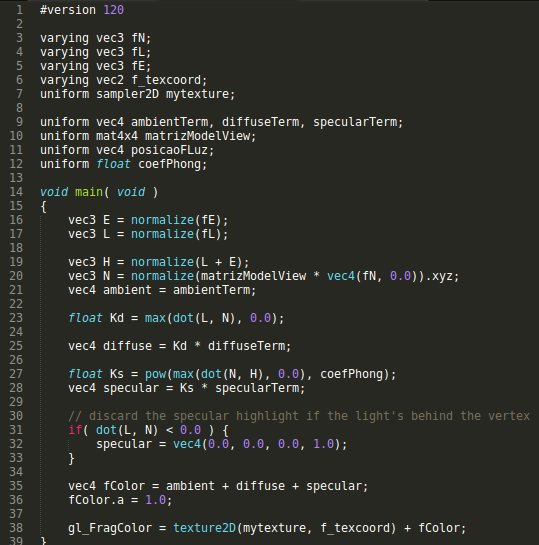
\includegraphics[width=230pt]{images/fragmentshader.png}}
\caption{Fragment Shader}
\label{img:complete}
\end{figure}

No fragment shader pode-se verificar que são usadas as variaveis passadas pelo Vertex Shader, neste caso, fE, fN e fL, calculando a respectiva cor do vertice, dando o efeito de iluminação pretendido.\\

Para realizar esta parte do código foi utilizado os slides dados na teórica das aulas de Computação Visual no ficheiro PDF ``Métodos de Iluminação e Sombreamento (PDF)'' disponível em \url{http://sweet.ua.pt/jmadeira/CV/CV_07_Ilumina%C3%A7%C3%A3o_e_Shading_BSS_JM.pdf} nos slides 50 a 53.\\

Ainda se pode verificar que as texturas são introduzidas com o texture2D que permite aplicar uma cor RGB a uma coordenada específica, fazendo isto com todas as coordendas, para além disto, ainda se pode verificar que dá-se igual importância a textura e a iluminação, apesar de não ser o melhor método funciona relativamente bem.

\section{Aspectos Importantes do Trabalho}

Os aspectos importantes deste trabalho vai desde a representação gráfica dos objectos (como peças de xadrez, texturas, skybox, movimentos possíveis de cada peça) e interacção com o utilizador (como clique nas peças de xadrez, teclado ou rato, e ainda manipulação da cena, teclado ou rato).

\subsection{Interacção com o utilizador}

\subsubsection{Clique nas peças do Xadrez (Interacção Directa)}

\subsubsection{Manipulação do cenário}

\subsection{Iluminação na Placa Gráfica}

\subsection{Texturas}

\subsection{Skybox}

\subsection{Representação Gráfica}

\subsubsection{Peças de Xadrez}

\subsubsection{Movimentos possíveis}

{\large Distinção de movimentos}

\subsubsection{Peças mortas}

\bibliography{adasd} % use a field named url or \url{} for URLs
% Note: the \bibliographystyle is set automatically

\end{document}
